 \let\negmedspace\undefined
\let\negthickspace\undefined
\documentclass[journal]{IEEEtran}
\usepackage[a5paper, margin=10mm, onecolumn]{geometry}
%\usepackage{lmodern} % Ensure lmodern is loaded for pdflatex
\usepackage{tfrupee} % Include tfrupee package

\setlength{\headheight}{1cm} % Set the height of the header box
\setlength{\headsep}{0mm}     % Set the distance between the header box and the top of the text

\usepackage{gvv-book}
\usepackage{gvv}
\usepackage{cite}
\usepackage{amsmath,amssymb,amsfonts,amsthm}
\usepackage{algorithmic}
\usepackage{graphicx}
\usepackage{textcomp}
\usepackage{xcolor}
\usepackage{txfonts}
\usepackage{listings}
\usepackage{enumitem}
\usepackage{mathtools}
\usepackage{gensymb}
\usepackage{comment}
\usepackage[breaklinks=true]{hyperref}
\usepackage{tkz-euclide} 
\usepackage{listings}
% \usepackage{gvv}                                        
\def\inputGnumericTable{}                                 
\usepackage[latin1]{inputenc}                                
\usepackage{color}                                            
\usepackage{array}                                            
\usepackage{longtable}                                       
\usepackage{calc}                                             
\usepackage{multirow}                                         
\usepackage{hhline}                                           
\usepackage{ifthen}                                           
\usepackage{lscape}
\begin{document}

\bibliographystyle{IEEEtran}
\vspace{3cm}

\title{1.6.10}
\author{EE25BTECH11060 - V.Namaswi}
% \maketitle
% \newpage
% \bigskip
{\let\newpage\relax\maketitle}

\renewcommand{\thefigure}{\theenumi}
\renewcommand{\thetable}{\theenumi}
\setlength{\intextsep}{10pt} % Space between text and floats
\textbf{Question}:\\
Show that the points $\vec{A}(1,-2,-8)$,$\vec{B}(5,0,-2)$ and $\vec{C}(11,3,7)$ are collinear and find the ratio in which B divides AC.

\bigskip


\textbf{Solution}:\\
 

\[
\begin{array}{|c|c|c|c|}
\hline
\textbf{Point} & \textbf{x} & \textbf{y} & \textbf{z} \\
\hline
A & 1 & -2 & -8 \\
B & 5 & 0 & -2 \\
C & 11 & 3 & 7 \\
\hline
\end{array}
\]


 collinearity matrix can be expressed as 

\begin{align*}
  \brak{B-A\;\;\;C-A} =\begin{myvec}{4  & 10\\2 & 5\\6  & 15}\end{myvec}
 \end{align*}\\

 \[
\begin{myvec}{4  & 10\\2 & 5\\6 & 15}\end{myvec}
\xleftrightarrow{R_3 \gets R_3-(R_1 + R_2)}
  \begin{myvec}{4  & 10\\2 & 5\\0 & 0}\end{myvec}
  \xleftrightarrow{R_1 \gets R_1-(2 R_2)} 
\begin{myvec}{0 & 0\\2 & 5\\0 & 0}\end{myvec}
\]

Which is a Rank 1 matrix , Hence   $\vec{A}(1,-2,-8)$,$\vec{B}(5,0,-2)$ and $\vec{C}(11,3,7)$ are collinear.\\

Section formula for a vector $\vec{B}$ which divides the line formed by vectors $\vec{A}$ and $\vec{C}$ in the ratio k:1 is given by

\begin{align}
    \vec{B}=\frac{k\vec{C}+\vec{A}}{k+1}\\
             \myvec{5\\0\\-2} &=\frac{{\myvec{1\\-2\\-8}+k\myvec{11\\3\\7}}}{1+k}\\
    \implies\myvec{5\\0\\-2} + k\myvec{5\\0\\-2} &=\myvec{1\\-2\\-8}+k\myvec{11\\3\\7}\\ 
    \implies \myvec{4 \\2 \\6} &= k\myvec{6 \\ 3 \\9}\\
    \implies k = \frac{2}{3}
\end{align}

 $\vec{B}$ which divides  $\vec{A}\vec{C}$ in the ratio 2:3


Refer to Fig. 0

\begin{figure}[H]
\begin{center}
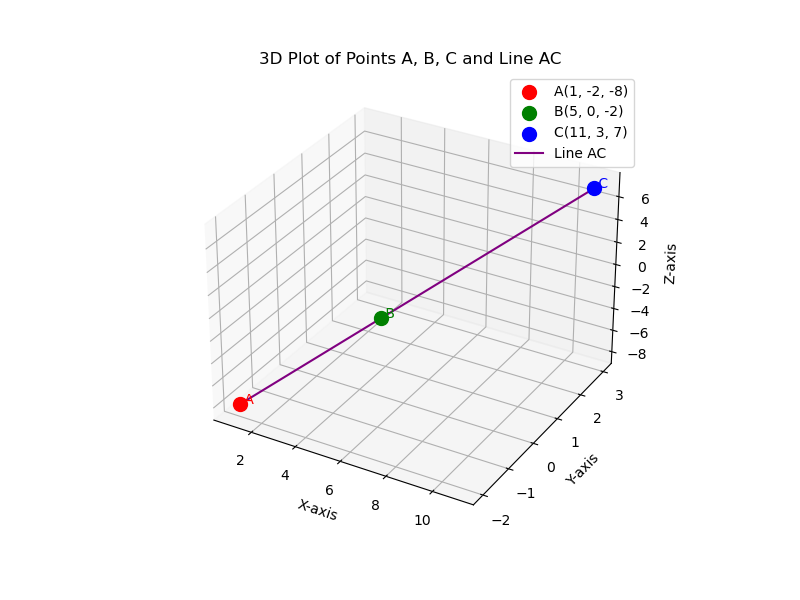
\includegraphics[width=0.6\columnwidth]{figs/Fig.png}
\end{center}
\caption{}
\label{fig:Fig}
\end{figure}


\end{document}